\documentclass[]{article}
\usepackage[utf8]{inputenc}
\usepackage[T1]{fontenc}
\usepackage{xcolor}
\usepackage{indentfirst}
\usepackage{hyperref}
\usepackage{graphicx}
\graphicspath{ {.} }
\usepackage{geometry}

\geometry{
	a4paper,
	total={170mm,257mm},
	left=20mm,
	top=20mm,
}
\hypersetup{
	colorlinks=true,
	linkcolor=blue,
	filecolor=magenta,      
	urlcolor=cyan,
}
%opening
\title{Obliczenia naukowe. Lista nr 2. Sprawozdanie.}
\author{Kacper Szatan, nr 236478}
\begin{document}
\maketitle
\section*{\centering CEL}
Celem listy jest zbadanie uwarunkowań napotkanych zadań oraz stabilności zastosowanych algorytmów.

Poniżej zajmiemy się omówieniem realizacji zadań wykonanych na drugie laboratorium. Przedstawimi również wyniki zaprezentowanych eksperymentów oraz wnioski jakie można wyciągnąć.
\section{Zadanie 1}
\subsection{Opis problemu}
W zadaniu pierwszym należy zastosować cztery algorytmy sumowania, które implementowaliśmy w zadaniu piątym na liście pierwszej. Algorytmy te mamy zastosować dla podanych wektorów danych:
\[\tilde{x} = [2.718281828, -3.141592654, 1.414213562, 0.577215664\sqcup, 0.301029995\sqcup]\]
\[y = [1486.2497, 878366.9879, -22.37492, 4773714.647, 0.000185049]\]
Różnica w danych między zadaniem piątym, a pierwszym polega na usunięciu ostatnich cyfr dla $x_4$ i $x_5$. 
\subsection{Realizacja}
Cztery algorytmy z zadania piątego z listy drugiej:
\begin{itemize}
	\item W przód.
	\item W tył.
	\item Od największego do najmniejszego. 
	\item Od najmniejszego do największego.
\end{itemize}
\newpage
\subsection{Wyniki}
\begin{table}[h]
	\centering
	\begin{tabular}{||c c c c||} 
		\hline
		Precyzja & Dane & Algorytm 1 & Algorytm 2\\ [0.5ex] 
		\hline\hline
		Float32 & $x$  & -0.4999443 &  -0.4543457\\ 
		Float32 & $\tilde{x}$ & -0.4999443 & -0.4543457\\
		Float64 & $x$ & 1.0251881368296672e-10 & -1.5643308870494366e-10\\
		Float64 & $\tilde{x}$ & -0.004296342739891585 &-0.004296342998713953\\
		\hline
		Prawidłowa wartość & \multicolumn{2}{c}{-1.00657107000000e-11}&\\
		\hline
	\end{tabular}
	\caption{Wynik sumowania przy zastosowaniu algorytmów w przód i w tył.}
\end{table}
\begin{table}[h]
	\centering
	\begin{tabular}{||c c c c||} 
		\hline
		Precyzja & Dane & Algorytm 3 & Algorytm 4 \\ [0.5ex] 
		\hline\hline
		Float32 & $x$ & -0.5 & -0.5\\ 
		Float32 & $\tilde{x}$ & -0.5 & -0.5\\
		Float64 & $x$ & 0.0 & 0.0\\
		Float64 & $\tilde{x}$ & -0.004296342842280865 & -0.004296342842280865\\
		\hline
		Prawidłowa wartość & \multicolumn{2}{c}{-1.00657107000000e-11}&\\
		\hline
	\end{tabular}
	\caption{Wynik sumowania przy zastosowaniu algorytmów od największego do najmniejszego i na odwrót.}
\end{table}
\subsection{Wnioski}
Od razu widać, że modyfikacja, której dokonaliśmy nie wpłynęła w ogóle na wyniki algorytmów przeprowadzanych w arytmetyce \textbf{FLOAT32}. Jest to spowodowane małą precyzją tej arytmetyki. Po zastosowaniu funkcji bitstring okazało się, że $\tilde{x_4} = x_4$ w arytmetyce \textbf{FLOAT32}, a $\tilde{x_5}$ różni się tylko na ostatnim najmniej znaczącym bicie w stosunku do $x_5$. Zatem nic dziwnego, że ta zmiana nie wpłyneła na wyniki algorytmów. Jednakże w arytmetyce \textbf{FLOAT64} po tej niewielkiej modyfikacji otrzymane wyniki drastycznie różnią się od tych przed modyfikacją danych. Pozwala nam to sądzić, że być może zadanie jest źle uwarunkowane. Aby potwierdzić nasze przypuszczenia możemy policzyć względną zmianę wyników z wzoru podanego na wykładzie:\[\frac{|f(x') - f(x)|}{|f(x)|} \]
Dla algorytmu w przód (pierwszej sumy) względna zmiana wyniku jest równa aż $4.19078478190021e7$ przy bardzo niewielkiej zmianie danych. Zatem nasze przypuszczenie o złym uwarunkowaniu zadania okazało się trafne.
\section{Zadanie 2}
\subsection{Opis problemu}
Zadanie polegało na narysowaniu wykresu funkcji: \[f(x)=e^xln(1 + e^{-x}
)\]
w co najmniej dwóch dowolnych programach do wizualizacji. Następnie należało policzyć granicę funkcji $\lim_{x\to\infty}f(x)$. Otrzymany wynik porównano z wykresami funkcji.
\subsection{Realizacja}
Podczas realizacji zdefiniowano w Julii zadaną funkcję, a następnię wyświetlono ją za pomocą trzech różnych "backendów" odpowiedzialnych za wizualizację. Do wyświetlenia posłużyły programy:
\begin{itemize}
	\item PyPlot
	\item UnicodePlots (drukuje tekstowy wykres w konsoli)
	\item InspectDr
\end{itemize}
Następnie wyliczono granicę z pomocą WolframAplha oraz analitycznie.

\subsection{Wyniki}
Wyliczenie granicy analitycznie:
\[\lim_{x\to\infty} e^x \ln(1 + e^{-x}) = \lim_{x\to\infty} \frac{\ln(1+e^{-x})}{e^{-x}} \rightarrow \frac{0}{0} \stackrel{H}{=}\]
\[\stackrel{H}{=} \lim_{x\to\infty} \frac{(\ln(1+e^{-x}))'}{(e^{-x})'} = \lim_{x\to\infty} \frac{\frac{1}{1+e^{-x}}(-e^{-x})}{-e^{-x}}= \lim_{x\to\infty} \frac{1}{1+e^{-x}} = 1\]
WolframAlpha również wyznacza tą granicę jako równą 1. 
\\\\
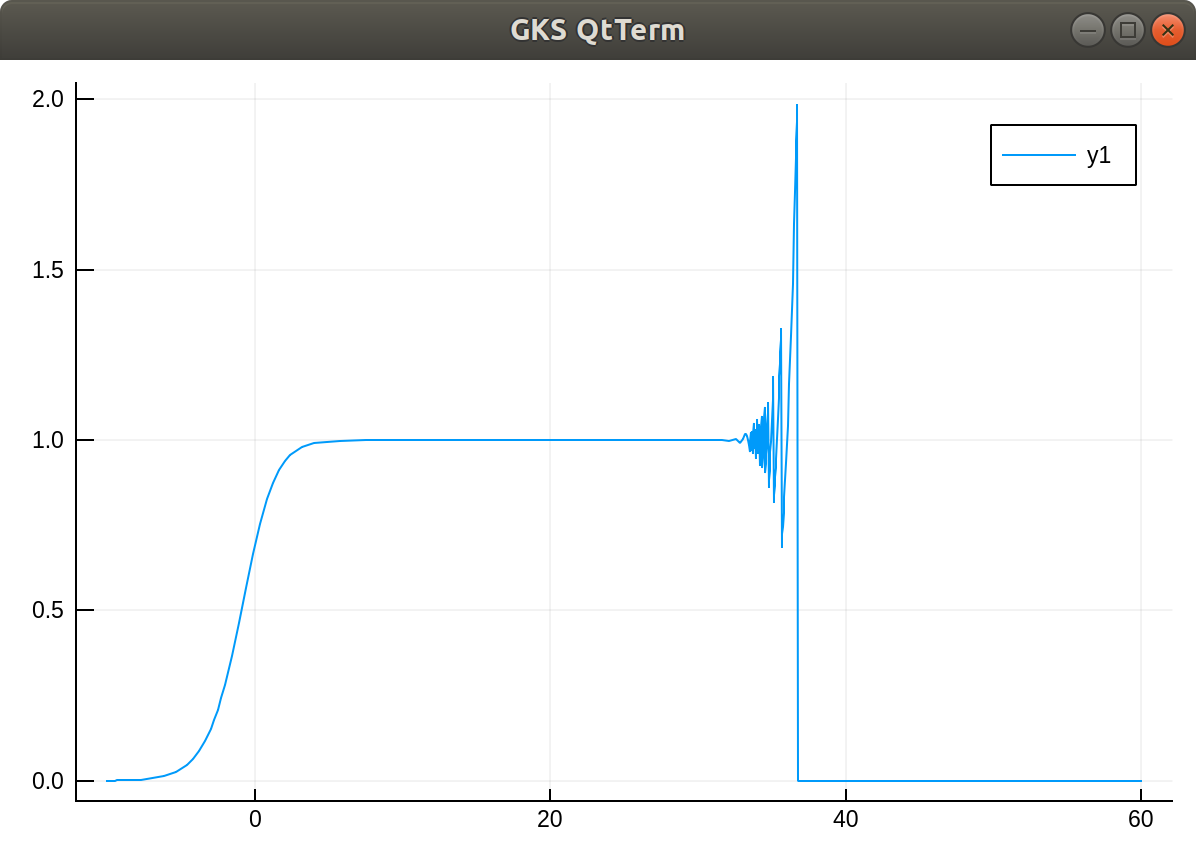
\includegraphics[scale=0.25]{PyPlotZad2.png}

\textit{Wykres 1: Wykres funckji $f$ stworzony za pomocą programu PyPlot.}
\\\\\\
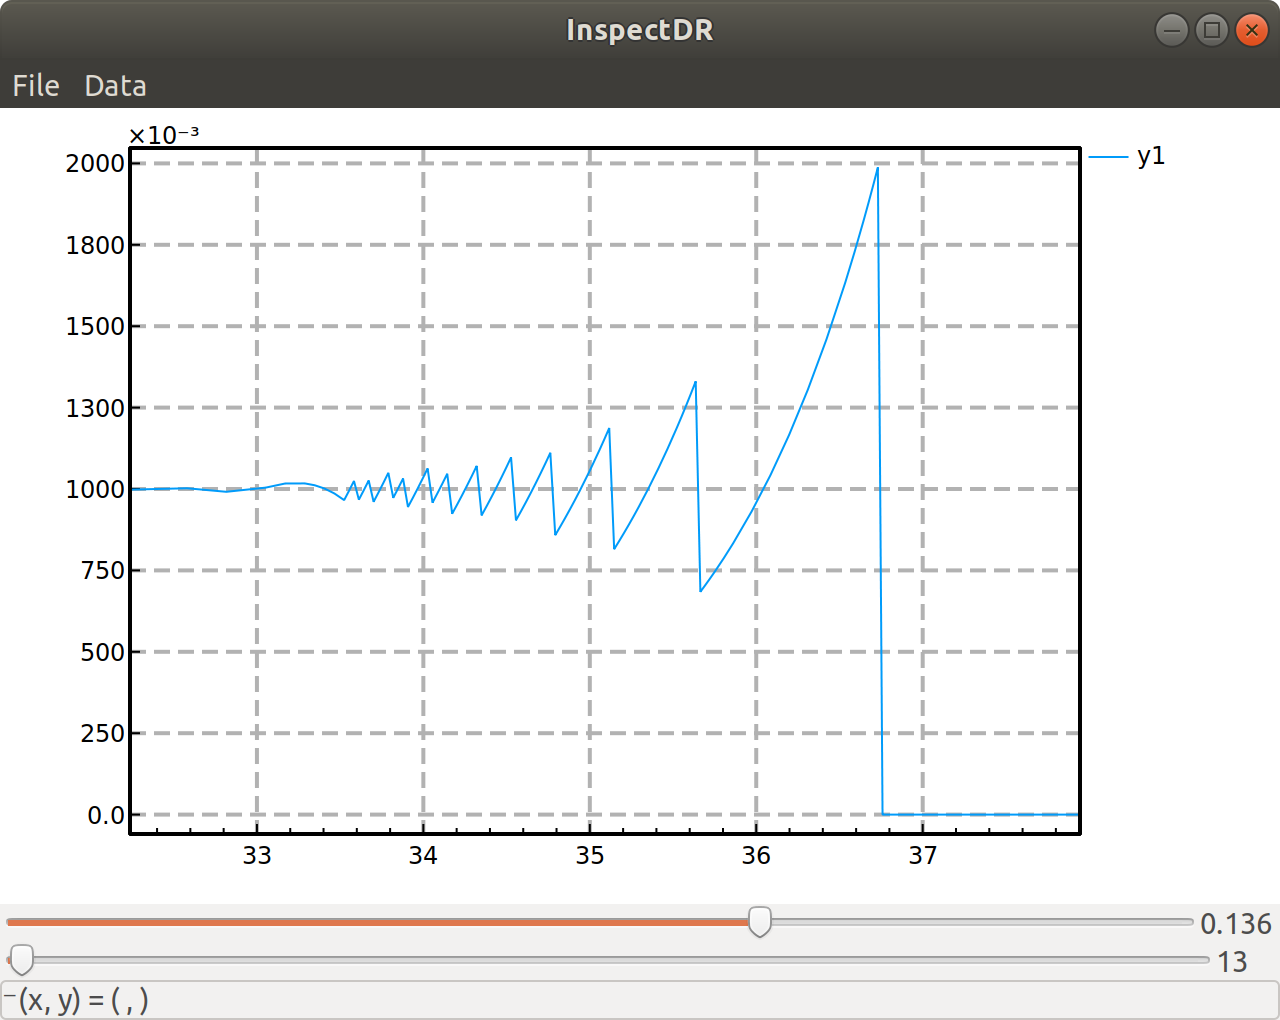
\includegraphics[scale=0.25]{InspectorDrZad2.png}

\textit{Wykres 2: Wykres funckji $f$ zbliżony w miejscu zaburzenia, stworzony za pomocą programu InspectDr.}
\newpage
\subsection{Wnioski}
Dokładna wyliczona przez nas i skonrolowana przez WolframAlpha granica wynosi 1. Niestety wykresy przez nas wygenerowane w okolicy $x = 33$ zaczynają się zaburzać, a dla $x$ bliskich 37 i większych wykres pokazuje już tylko zero. Jest to najpewniej spowodowane pochłanianiem małych wartości $e^{-x}$ przez jedynkę w logarytmie. To prowadzi do przybliżenia sumy w logarytmie. Następnie ten mały błąd pomnożony przez bardzo dużą liczbę $e^x$ zwielokrotnia nam błąd wynikający z zakrągleń arytmetki. Dla większych wartości $x$ wykresy pokazują, wartość funkcji równą 0. Dzieje się tak, bo suma w logarytmie $1+e^{-x} = 1$ dla $x$ bliskiego 37 i większych. Stąd mamy, że wynikiem logarytmu jest zero, a zero razy cokolwiek da nam zero. Chyba, że z $x$ dojdziemy do takiej wartości, że $e^x = Inf$. Wtedy julia zwróci nam NaN, ponieważ 0.0 * Inf = NaN.
\section{Zadanie 3}
\subsection{Opis problemu}
W zadaniu trzecim należało rozwiązać równanie $\mathbf{Ax = b}$ dla macierzy współczynników $\mathbf{A} \epsilon \mathcal{R}^{n \times n}$ i wektora prawych stron $\mathbf{b} \epsilon \mathcal{R}^{n}$. Macierz $\mathbf{A}$ generowaliśmy na dwa sposoby:
\begin{itemize}
	\item jako macierz Hilberta stopnia $n$.
	\item jako macierz losowa stopnia $n$ i z zadanym wskaźnikiem uwarunkowania $c$. 
\end{itemize}
Wektor $\mathbf{b}$ jest zadany jako $\mathbf{b = Ax}$ przy czym $\mathbf{x} = (1,...,1)^{T}$, żeby było znane dokładne rozwiązanie. Równanie mamy rozwiązać przy pomocy dwóch algorytmów:
\begin{itemize}
	\item eliminacja Gaussa $\mathbf{x = A \backslash b}$.
	\item macierz odwrotna $\mathbf{x = A^{-1} b}$
\end{itemize}
\subsection{Realizacja}
Wygenerowano macierze hilberta $\mathbf{H_n}$ dla stopnia $\mathbf{n} \epsilon [2, 3, ..., 20]$ za pomocą dostarczonych źródeł z hilb.jl. Plik matcond.jl pozwolił na stworzenie losowych macierzy $\mathbf{R^c_n}$ dla stopnia $\mathbf{n} \epsilon [5, 10, 20]$ i rosnącego wskaźnika uwarunkowania $\mathbf{c} \epsilon [1, 10, 10^3, 10^7, 10^{12}, 10^{16} ]$. Następnie rozwiązano równanie dla każdej macierzy dwoma metodami (Gauss, Inversion). Na końcu wyliczono jeszcze błąd względny uzyskanych wyników korzystając ze wzoru $ \frac{||x - \tilde{x} ||}{||x||}$. Dzięki pakietowi LinearAlgebra określano jeszcze rząd obliczonej macierzy oraz jej wskaźnik uwarunkowania. 
\newpage
\subsection{Wyniki}
\begin{table}[h]
	\centering
	\begin{tabular}{||c c c c c||} 
		\hline
		Stopień & Rząd & Cond & Gauss(error) & Inversion(error) \\ [0.5ex] 
		\hline\hline
		2 & 2 & 19.28147006790397 & 5.661048867003676e-16 & 1.4043333874306803e-15 \\
		3 & 3 & 524.0567775860644 & 8.022593772267726e-15 & 0.0 \\
		4 & 4 & 15513.73873892924 & 4.137409622430382e-14 & 0.0 \\
		5 & 5 & 476607.25024259434 & 1.6828426299227195e-12 & 3.3544360584359632e-12 \\
		6 & 6 & 1.4951058642254665e7 & 2.618913302311624e-10 & 2.0163759404347654e-10 \\
		7 & 7 & 4.75367356583129e8 & 1.2606867224171548e-8 & 4.713280397232037e-9 \\
		8 & 8 & 1.5257575538060041e10 & 6.124089555723088e-8 & 3.07748390309622e-7 \\
		9 & 9 & 4.931537564468762e11 & 3.8751634185032475e-6 & 4.541268303176643e-6 \\
		10 & 10 & 1.6024416992541715e13 & 8.67039023709691e-5 & 0.0002501493411824886 \\
		11 & 10 & 5.222677939280335e14 & 0.00015827808158590435 & 0.007618304284315809 \\
		12 & 11 & 1.7514731907091464e16 & 0.13396208372085344 & 0.258994120804705 \\
		13 & 11 & 3.344143497338461e18 & 0.11039701117868264 & 5.331275639426837 \\
		14 & 11 & 6.200786263161444e17 & 1.4554087127659643 & 8.71499275104814 \\
		15 & 12 & 3.674392953467974e17 & 4.696668350857427 & 7.344641453111494 \\
		16 & 12 & 7.865467778431645e17 & 54.15518954564602 & 29.84884207073541 \\
		17 & 12 & 1.263684342666052e18 & 13.707236683836307 & 10.516942378369349 \\
		18 & 12 & 2.2446309929189128e18 & 9.134134521198485 & 7.575475905055309 \\
		19 & 13 & 6.471953976541591e18 & 9.720589712655698 & 12.233761393757726 \\
		20 & 13 & 1.3553657908688225e18 & 7.549915039472976 & 22.062697257870493 \\
		\hline
	\end{tabular}
	\caption{Wyniki przeprowadzonych eksperymentów dla macierzy Hilberta.}
\end{table}

\begin{table}[h]
	\centering
	\begin{tabular}{||c c c c c||} 
		\hline
		Stopień & Rząd & Cond & Gauss(error) & Inversion(error) \\ [0.5ex] 
		\hline\hline
		5 & 5 & 1.0 & 1.5700924586837752e-16 & 1.9860273225978183e-16 \\
		5 & 5 & 10.0 & 4.965068306494546e-17 & 2.482534153247273e-16 \\
		5 & 5 & 1000.0 & 3.8130948794063295e-14 & 3.3816161346438753e-14 \\
		5 & 5 & 1.0e7 & 2.2919927882791603e-10 & 2.2953311159660053e-10 \\
		5 & 5 & 1.0e12 & 9.930136612989092e-17 & 1.1819407184470875e-5 \\
		5 & 4 & 1.0e16 & 0.38298628154598324 & 0.36255387530682937 \\
		10 & 10 & 1.0 & 2.328823463338184e-16 & 4.0792198665315547e-16 \\
		10 & 10 & 10.0 & 2.5559253454202263e-16 & 2.895107444979072e-16 \\
		10 & 10 & 1000.0 & 1.3703768418523405e-14 & 1.8361356958809712e-14 \\
		10 & 10 & 1.0e7 & 9.753013305378921e-11 & 1.438359473034689e-10 \\
		10 & 10 & 1.0e12 & 3.932920195316686e-5 & 3.597703968961513e-5 \\
		10 & 9 & 1.0e16 & 0.7572965466871276 & 0.7589151128008322 \\
		20 & 20 & 1.0 & 5.370542509574173e-16 & 4.74936748511455e-16 \\
		20 & 20 & 10.0 & 5.600852339972845e-16 & 4.0183325713214166e-16 \\
		20 & 20 & 1000.0 & 1.476680095807448e-14 & 1.9246029150100703e-14 \\
		20 & 20 & 1.0e7 & 1.6573334702084863e-10 & 1.658199909023172e-10 \\
		20 & 20 & 1.0e12 & 2.1119180994645343e-5 & 1.3131648619124226e-5 \\
		20 & 19 & 1.0e16 & 0.4019205888419031 & 0.371337553547061 \\
		\hline
	\end{tabular}
	\caption{Wyniki przeprowadzonych eksperymentów dla macierzy losowych zadanym wskaźnikiem uwarunkowania.}
\end{table}
\subsection{Wnioski}
Analizując wyniki łatwo zauważyć, że wielkość błędu względnego jest mocno skorelowana z wskaźnikiem uwarunkowania macierzy. Im większy wskaźnik tym większy błąd jest popełniany dlatego zadania w których operujemy na macierzach z wysokim wskaźnikiem uwarunkowania są źle uwarunkowane. Ponadto można zauważyć, że wskaźnik uwarunkowania macierzy Hilberta rośnie bardzo szybko wraz z wzrostem ich stopnia (rozmiaru). Przy obliczaniu zadań, w których mamy doczynienia z macierzą Hilberta, powinniśmy stosować algorytm eliminacji Gaussa, który popełnia mniejszy błąd niż alogrytm odwracający macierz.
\section{Zadanie 4}
\subsection{Opis problemu}
Zadanie polegało na obliczeniu 20 miejsc zerowych wielomianu $P$, który jest wielomianem Wilkinsona w postaci naturalnej. Wielomian Wilkinsona będziemy oznaczać przez $p$. Następnie należało sprawdzić wyliczone pierwiastki $z_k : k \epsilon [1, 2, ... , 20]$ przez obliczenie $|P(z_k)|$, $|p(z_k)|$ oraz $|z_k - k|$. Powstałe rozbieżności omówić. W drugim podpunktcie należło przerpowadzić eksperyment jeszcze raz, ale tym razem dla lekko zmodyfikowanego wielomianu $P$ i wyjaśnić powstałe różnice. 
\subsection{Realizacja}
Za pomocą pakietu Polynomials utworzono wielomian $P$ korzystając z funkcji \textit{Poly}. Utworzono też wielomian Wilkinsona $p$ za pomocą funkcji \textit{poly}. Policzono miejsca zerowe wielomianu $P$ za pomocą funkcji roots. Następnie funkcja \textit{polyval} posłużyła do wyliczenia wartości wielomianów $P$ i $p$ w wyliczonych wcześniej miejscach zerowych. Obliczono również błąd bezwzględny między obliczonymi miejscami zerowymi, a ich faktyczną wartością. Następnie powtórzono cały eksperyment dla wielomianu zaburzonego o wartość $-2^{-23}$ przy wyrazie $x^19$.  
\subsection{Wyniki}
Przedstawiono na tabelach 5, 6 i 7.
\begin{table}[h]
	\centering
	\begin{tabular}{||c c c c c||} 
		\hline
		$k$ & $|P(z_k)|$ & $|p(z_k)|$ & $|z_k - k|$ & $z_k$ \\ [0.5ex] 
		\hline\hline
		1 & 36352.0 & 38400.0 & 3.0109248427834245e-13 & 0.9999999999996989 \\
		2 & 181760.0 & 198144.0 & 2.8318236644508943e-11 & 2.0000000000283182 \\
		3 & 209408.0 & 301568.0 & 4.0790348876384996e-10 & 2.9999999995920965 \\
		4 & 3.106816e6 & 2.844672e6 & 1.626246826091915e-8 & 3.9999999837375317 \\
		5 & 2.4114688e7 & 2.3346688e7 & 6.657697912970661e-7 & 5.000000665769791 \\
		6 & 1.20152064e8 & 1.1882496e8 & 1.0754175226779239e-5 & 5.999989245824773 \\
		7 & 4.80398336e8 & 4.78290944e8 & 0.00010200279300764947 & 7.000102002793008 \\
		8 & 1.682691072e9 & 1.67849728e9 & 0.0006441703922384079 & 7.999355829607762 \\
		9 & 4.465326592e9 & 4.457859584e9 & 0.002915294362052734 & 9.002915294362053 \\
		10 & 1.2707126784e10 & 1.2696907264e10 & 0.009586957518274986 & 9.990413042481725 \\
		11 & 3.5759895552e10 & 3.5743469056e10 & 0.025022932909317674 & 11.025022932909318 \\
		12 & 7.216771584e10 & 7.2146650624e10 & 0.04671674615314281 & 11.953283253846857 \\
		13 & 2.15723629056e11 & 2.15696330752e11 & 0.07431403244734014 & 13.07431403244734 \\
		14 & 3.65383250944e11 & 3.653447936e11 & 0.08524440819787316 & 13.914755591802127 \\
		15 & 6.13987753472e11 & 6.13938415616e11 & 0.07549379969947623 & 15.075493799699476 \\
		16 & 1.555027751936e12 & 1.554961097216e12 & 0.05371328339202819 & 15.946286716607972 \\
		17 & 3.777623778304e12 & 3.777532946944e12 & 0.025427146237412046 & 17.025427146237412 \\
		18 & 7.199554861056e12 & 7.1994474752e12 & 0.009078647283519814 & 17.99092135271648 \\
		19 & 1.0278376162816e13 & 1.0278235656704e13 & 0.0019098182994383706 & 19.00190981829944 \\
		20 & 2.7462952745472e13 & 2.7462788907008e13 & 0.00019070876336257925 & 19.999809291236637 \\
		\hline
	\end{tabular}
	\caption{Wyniki przeprowadzonych eksperymentów dla wielomianu Wilkinsona.}
\end{table}

\begin{table}[h]
	\centering
	\begin{tabular}{||c c c c||} 
		\hline
		$k$ & $|P(z_k)|$ & $|p(z_k)|$ & $|z_k - k|$\\ [0.5ex] 
		\hline\hline
		1 & 20992.0 & 22016.0 & 1.6431300764452317e-13\\
		2 & 349184.0 & 365568.0 & 5.503730804434781e-11\\
		3 & 2.221568e6 & 2.295296e6 & 3.3965799062229962e-9\\
		4 & 1.046784e7 & 1.0729984e7 & 8.972436216225788e-8\\
		5 & 3.9463936e7 & 4.3303936e7 & 1.4261120897529622e-6\\
		6 & 1.29148416e8 & 2.06120448e8 & 2.0476673030955794e-5\\
		7 & 3.88123136e8 & 1.757670912e9 & 0.00039792957757978087\\
		8 & 1.072547328e9 & 1.8525486592e10 & 0.007772029099445632\\
		9 & 3.065575424e9 & 1.37174317056e11 & 0.0841836320674414\\
		10 & 7.143113638035824e9 & 1.4912633816754019e12 & 0.6519586830380406\\
		11 & 7.143113638035824e9 & 1.4912633816754019e12 & 1.1109180272716561\\
		12 & 3.357756113171857e10 & 3.2960214141301664e13 & 1.665281290598479\\
		13 & 3.357756113171857e10 & 3.2960214141301664e13 & 2.045820276678428\\
		14 & 1.0612064533081976e11 & 9.545941595183662e14 & 2.5188358711909045\\
		15 & 1.0612064533081976e11 & 9.545941595183662e14 & 2.7128805312847097\\
		16 & 3.315103475981763e11 & 2.7420894016764064e16 & 2.9060018735375106\\
		17 & 3.315103475981763e11 & 2.7420894016764064e16 & 2.825483521349608\\
		18 & 9.539424609817828e12 & 4.2525024879934694e17 & 2.454021446312976\\
		19 & 9.539424609817828e12 & 4.2525024879934694e17 & 2.004329444309949\\
		20 & 1.114453504512e13 & 1.3743733197249713e18 & 0.8469102151947894\\
		\hline
	\end{tabular}
	\caption{Wyniki przeprowadzonych eksperymentów dla \textbf{zaburzonego} wielomianu Wilkinsona.}
\end{table}

\begin{table}[h!]
	\centering
	\begin{tabular}{||c||} 
		\hline
		$z_k$\\ [0.5ex] 
		\hline\hline
		0.9999999999998357 + 0.0im \\
		2.0000000000550373 + 0.0im \\
		2.99999999660342 + 0.0im \\
		4.000000089724362 + 0.0im \\
		4.99999857388791 + 0.0im \\
		6.000020476673031 + 0.0im \\
		6.99960207042242 + 0.0im \\
		8.007772029099446 + 0.0im \\
		8.915816367932559 + 0.0im \\
		10.095455630535774 - 0.6449328236240688im \\
		10.095455630535774 + 0.6449328236240688im \\
		11.793890586174369 - 1.6524771364075785im \\
		11.793890586174369 + 1.6524771364075785im \\
		13.992406684487216 - 2.5188244257108443im \\
		13.992406684487216 + 2.5188244257108443im \\
		16.73074487979267 - 2.812624896721978im \\
		16.73074487979267 + 2.812624896721978im \\
		19.5024423688181 - 1.940331978642903im \\
		19.5024423688181 + 1.940331978642903im \\
		20.84691021519479 + 0.0im \\
		\hline
	\end{tabular}
	\caption{Miejsca zerowe \textbf{zaburzonego} wielomianu Wilkinsona.}
\end{table}
\subsection{Wnioski}
Analizując jedynie kolumnę z błędem bezwzględnym możemy dojść do mylnego przekonania, że pierwiastki wielomianu zostały prawidłowo wyliczone gdyż popełniony błąd jest niewielki. Jednakże gdy popatrzymy na wartości wielomianów w obliczonych miejscach zerowych to okaże się, że są one dalekie od $0$. W pewnym momencie przekraczają one nawet bilion. Gwałtowny wzrost odchylenia w wyliczeniach $P(z_k)$ i $p(z_k)$ jest spowodowany tym, że nawet małe odchylenie w wyliczeniu pierwiastka jest mnożone przez bardzo duży czynik wielkości $19!$. Błąd przy wyliczeniach miejsc zerowych powodowany jest przez to, że wspołczynniki w wielomianie Wilkinsona mają nawet 19 cyfr znaczących, a w języku julia, w arytmetyce Float64 jesteśmy wstanie dokładnie reprezentować od 15 do 17 cyfr w systemie dziesiętnym.

Wielomian $p$ wyliczany za pomocną funkcji \textit{poly} (forma iloczynowa) jest nieznacznie dokładniejszy gdyż daje wyniki bliższe zeru niż wielomian $P$ jednakże są one tego samego rzędu. Zatem jest to niezbyt znacząc różnica.

Gdy eksperyment przeprowadzono po małej modyfikacji współczynnika, części miejsc zerowych była liczbami zespolonymi.

Omówione odkształcenia wynikiów potwierdzają iż poroblem obliczania miejsc zerowych wielomianu Wilkinsona jest zadaniem źle uwarunkowanym (mała modyfikacja danych doprowadziła do dużego odkształcenia wyników).  
\section{Zadanie 5}
\subsection{Opis problemu}
W zadaniu piątym mieliśmy poddać rozważaniu model logistyczny wzrostu populacji. \[p_{n+1} := p_n + rp_n(1-p_n), n = 0, 1, ...\] W modelu tym $r$ jest pewną daną stałą, a $r(1-p_n)$ jest czynnikiem wzrostu populacji. Natomiast $p_0$ jest wielkością populacji stanowiąca procent maksymalnej wielkości populacji dla danego stanu środowiska. Przeprowadzono dwa eksperymenty polegające na wykonaniu 40 iteracji rekurencyjnego wyrażenia opisującego nasz model. W pierwszym eksperymencie zastosowano obcięcie wyniku do 3 cyfr po przecinku po 10 iteracji. Ekspeyment pierwszy prowadzony był w arytmetyce \textbf{Float32}, a eksperyment drugi w \textbf{Float32} i \textbf{Float64}. W naszych eksperymentach stała $r = 3$, a $p_0 = 0.01$.  
\subsection{Realizacja}
Opracowano funkcje, która umożliwia przeprowadzenie obu eksperymentów. Gdy podamy odpowiednią flagę w jej argumencie pozwala ona na opcjonalne obcięcie cyfr znaczących po dziesiątej iteracji. Funkcja ta zapewnia prawidłowe wykonywanie operacji w zadanej arytmetyce.
\subsection{Wyniki}
\begin{table}[h!]
	\centering
	\begin{tabular}{||c c c c||} 
		\hline
		Iteracja & Zmodyfikowany \textbf{Float32} & \textbf{Float32} & \textbf{Float64} \\ [0.5ex] 
		\hline\hline
		0 & 0.01 & 0.01 & 0.01 \\
		1 & 0.0397 & 0.0397 & 0.0397 \\
		2 & 0.15407173 & 0.15407173 & 0.15407173000000002 \\
		3 & 0.5450726 & 0.5450726 & 0.5450726260444213 \\
		4 & 1.2889781 & 1.2889781 & 1.2889780011888006 \\
		5 & 0.1715188 & 0.1715188 & 0.17151914210917552 \\
		6 & 0.5978191 & 0.5978191 & 0.5978201201070994 \\
		7 & 1.3191134 & 1.3191134 & 1.3191137924137974 \\
		8 & 0.056273222 & 0.056273222 & 0.056271577646256565 \\
		9 & 0.21559286 & 0.21559286 & 0.21558683923263022 \\
		\textbf{10} & \textbf{0.722} &  0.7229306 & 0.722914301179573 \\
		11 & 1.3241479 & 1.3238364 & 1.3238419441684408 \\
		12 & 0.036488414 & 0.037716985 & 0.03769529725473175 \\
		13 & 0.14195944 & 0.14660022 & 0.14651838271355924 \\
		14 & 0.50738037 & 0.521926 & 0.521670621435246 \\
		15 & 1.2572169 & 1.2704837 & 1.2702617739350768 \\
		16 & 0.28708452 & 0.2395482 & 0.24035217277824272 \\
		17 & 0.9010855 & 0.7860428 & 0.7881011902353041 \\
		18 & 1.1684768 & 1.2905813 & 1.2890943027903075 \\
		19 & 0.577893 & 0.16552472 & 0.17108484670194324 \\
		20 & 1.3096911 & 0.5799036 & 0.5965293124946907 \\
		21 & 0.09289217 & 1.3107498 & 1.3185755879825978 \\
		22 & 0.34568182 & 0.088804245 & 0.058377608259430724 \\
		23 & 1.0242395 & 0.3315584 & 0.22328659759944824 \\
		24 & 0.94975823 & 0.9964407 & 0.7435756763951792 \\
		25 & 1.0929108 & 1.0070806 & 1.315588346001072 \\
		26 & 0.7882812 & 0.9856885 & 0.07003529560277899 \\
		27 & 1.2889631 & 1.0280086 & 0.26542635452061003 \\
		28 & 0.17157483 & 0.9416294 & 0.8503519690601384 \\
		29 & 0.59798557 & 1.1065198 & 1.2321124623871897 \\
		30 & 1.3191822 & 0.7529209 & 0.37414648963928676 \\
		31 & 0.05600393 & 1.3110139 & 1.0766291714289444 \\
		32 & 0.21460639 & 0.0877831 & 0.8291255674004515 \\
		33 & 0.7202578 & 0.3280148 & 1.2541546500504441 \\
		34 & 1.3247173 & 0.9892781 & 0.29790694147232066 \\
		35 & 0.034241438 & 1.021099 & 0.9253821285571046 \\
		36 & 0.13344833 & 0.95646656 & 1.1325322626697856 \\
		37 & 0.48036796 & 1.0813814 & 0.6822410727153098 \\
		38 & 1.2292118 & 0.81736827 & 1.3326056469620293 \\
		39 & 0.3839622 & 1.2652004 & 0.0029091569028512065 \\
		40 & 1.093568 & 0.25860548 & 0.011611238029748606 \\
		\hline
	\end{tabular}
	\caption{Wyniki iteracji modelu logistycznego w dwóch przeprowadzonych eksperymentach.}
\end{table}
\subsection{Wnioski}
Porównując wyniki rekurencji zmodyfikowanej i tej niezmodyfikowanej w arytmetyce \textbf{Float32} można zaobserwować, że po zastosowaniu obcięcia zaczynają one się "rozjeżdżać". Jako, że mamy doczynienia z problemem, w którym wyjście jednej iteracji stanowi wejście następnej to nie należy się dziwić "wzrostem" różnicy w wynikach w kolejnych iteracjach. Mimo, że początkowy błąd powodowany przez obcięcie jest niewielki to w każdej iteracji jest on powiększany. Z tych samych powodów podczas drugiego eksperymentu wyniki we \textbf{Float64} są tak bardzo różne od \textbf{Float32}. Tylko, że w eksperymencie drugim popełniamy ciągły błąd przez różnicę w długości mantys tych arytmetyk. Już dla trzeciej iteracji otrzymujemy różne dane na wejściu, stąd tak duże rozbieżności w wynikach, w póżniejszych iteracjach. Tak na prawdę, żadna z arytmetyk nie daje nam pewności co do dobrych wyników. Jak wiemy z poprzedniego zadania we \textbf{Float64} dokładne jest maksymalnie 17 cyfr w systemie dziesiętnym. A niektóre wyniki są dłuższe. Zatem i tak popełniamy błąd zapisu, a następnie przekazujemy ten błędny wynik jako wejście kolejnej itertacji gdzie zostatenie on powiększony. Zatem możemy powiedzieć, że ten algorytm jest niestabilny.     
\section{Zadanie 6}
\subsection{Opis problemu}
W ostatnim zadaniu należało rozważyć równanie rekurencyjne \[x_{n+1} := x^2_n + c, n = 0, 1, ...\]
Należało przeprowadzić 40 iteracji tego równania dla następujących warunków:
\begin{itemize}
	\item[a$)$] $c = -2$ i $x_0 = 1$
	\item[b$)$] $c = -2$ i $x_0 = 2$
	\item[c$)$] $c = -2$ i $x_0 = 1.99999999999999$
	\item[d$)$] $c = -1$ i $x_0 = 1$
	\item[e$)$] $c = -1$ i $x_0 = -1$
	\item[f$)$] $c = -1$ i $x_0 = 0.75$
	\item[g$)$] $c = -1$ i $x_0 = 0.25$
\end{itemize}

\subsection{Realizacja}
Obliczenia prowadzono w arytmetyce \textbf{Float64}. Skonstruowano funkcje rekurencyjną, która pozwala na 40 iteracji i zapisuje wyniki do podanej tablicy aby można je było łatwo odczytać. Skorzystano też z InspectDR aby zwizualizować wylilczone ciągi. Poniżej podano wykresy dla ciągu \textit{c, f i g}.
\newpage
\subsection{Wyniki}
\begin{table}[h!]
	\centering
	\begin{tabular}{||c c c c c c c c||} 
		\hline
		iteracja \vline & \multicolumn{3}{c}{$c = -2$} \vline & \multicolumn{4}{c||}{$c = -1$}  \\ [0.25ex]
		\hline		 
		$x_0 =>$ & 1.0 & 2.0 & 1.99999999999999 & 1.0 & -1.0 & 0.75 & 0.25 \\
		\hline\hline
		1 & -1.0 & 2.0 & 1.99999999999996 & 0.0 & 0.0 & -0.4375 & -0.9375 \\
		2 & -1.0 & 2.0 & 1.9999999999998401 & -1.0 & -1.0 & -0.80859375 & -0.12109375 \\
		3 & -1.0 & 2.0 & 1.9999999999993605 & 0.0 & 0.0 & -0.3461761474609375 & -0.9853363037109375 \\
		4 & -1.0 & 2.0 & 1.999999999997442 & -1.0 & -1.0 & -0.8801620749291033 & -0.029112368589267135 \\
		5 & -1.0 & 2.0 & 1.9999999999897682 & 0.0 & 0.0 & -0.2253147218564956 & -0.9991524699951226 \\
		6 & -1.0 & 2.0 & 1.9999999999590727 & -1.0 & -1.0 & -0.9492332761147301 & -0.0016943417026455965\\
		7 & -1.0 & 2.0 & 1.999999999836291 & 0.0 & 0.0 & -0.0989561875164966 & -0.9999971292061947 \\
		8 & -1.0 & 2.0 & 1.9999999993451638 & -1.0 & -1.0 & -0.9902076729521999 & -5.741579369278327e-6 \\
		9 & -1.0 & 2.0 & 1.9999999973806553 & 0.0 & 0.0 & -0.01948876442658909 & -0.9999999999670343 \\
		10 & -1.0 & 2.0 & 1.999999989522621 & -1.0 & -1.0 & -0.999620188061125 & -6.593148249578462e-11 \\
		11 & -1.0 & 2.0 & 1.9999999580904841 & 0.0 & 0.0 & -0.0007594796206411569 & -1.0 \\
		12 & -1.0 & 2.0 & 1.9999998323619383 & -1.0 & -1.0 & -0.9999994231907058 & 0.0 \\
		13 & -1.0 & 2.0 & 1.9999993294477814 & 0.0 & 0.0 & -1.1536182557003727e-6 & -1.0 \\
		14 & -1.0 & 2.0 & 1.9999973177915749 & -1.0 & -1.0 & -0.9999999999986692 & 0.0 \\
		15 & -1.0 & 2.0 & 1.9999892711734937 & 0.0 & 0.0 & -2.6616486792363503e-12 & -1.0 \\
		16 & -1.0 & 2.0 & 1.9999570848090826 & -1.0 & -1.0 & -1.0 & 0.0 \\
		17 & -1.0 & 2.0 & 1.999828341078044 & 0.0 & 0.0 & 0.0 & -1.0 \\
		18 & -1.0 & 2.0 & 1.9993133937789613 & -1.0 & -1.0 & -1.0 & 0.0 \\
		19 & -1.0 & 2.0 & 1.9972540465439481 & 0.0 & 0.0 & 0.0 & -1.0 \\
		20 & -1.0 & 2.0 & 1.9890237264361752 & -1.0 & -1.0 & -1.0 & 0.0 \\
		21 & -1.0 & 2.0 & 1.9562153843260486 & 0.0 & 0.0 & 0.0 & -1.0 \\
		22 & -1.0 & 2.0 & 1.82677862987391 & -1.0 & -1.0 & -1.0 & 0.0 \\
		23 & -1.0 & 2.0 & 1.3371201625639997 & 0.0 & 0.0 & 0.0 & -1.0 \\
		24 & -1.0 & 2.0 & -0.21210967086482313 & -1.0 & -1.0 & -1.0 & 0.0 \\
		25 & -1.0 & 2.0 & -1.9550094875256163 & 0.0 & 0.0 & 0.0 & -1.0 \\
		26 & -1.0 & 2.0 & 1.822062096315173 & -1.0 & -1.0 & -1.0 & 0.0 \\
		27 & -1.0 & 2.0 & 1.319910282828443 & 0.0 & 0.0 & 0.0 & -1.0 \\
		28 & -1.0 & 2.0 & -0.2578368452837396 & -1.0 & -1.0 & -1.0 & 0.0 \\
		29 & -1.0 & 2.0 & -1.9335201612141288 & 0.0 & 0.0 & 0.0 & -1.0 \\
		30 & -1.0 & 2.0 & 1.7385002138215109 & -1.0 & -1.0 & -1.0 & 0.0 \\
		31 & -1.0 & 2.0 & 1.0223829934574389 & 0.0 & 0.0 & 0.0 & -1.0 \\
		32 & -1.0 & 2.0 & -0.9547330146890065 & -1.0 & -1.0 & -1.0 & 0.0 \\
		33 & -1.0 & 2.0 & -1.0884848706628412 & 0.0 & 0.0 & 0.0 & -1.0 \\
		34 & -1.0 & 2.0 & -0.8152006863380978 & -1.0 & -1.0 & -1.0 & 0.0 \\
		35 & -1.0 & 2.0 & -1.3354478409938944 & 0.0 & 0.0 & 0.0 & -1.0 \\
		36 & -1.0 & 2.0 & -0.21657906398474625 & -1.0 & -1.0 & -1.0 & 0.0 \\
		37 & -1.0 & 2.0 & -1.953093509043491 & 0.0 & 0.0 & 0.0 & -1.0 \\
		38 & -1.0 & 2.0 & 1.8145742550678174 & -1.0 & -1.0 & -1.0 & 0.0 \\
		39 & -1.0 & 2.0 & 1.2926797271549244 & 0.0 & 0.0 & 0.0 & -1.0 \\
		40 & -1.0 & 2.0 & -0.3289791230026702 & -1.0 & -1.0 & -1.0 & 0.0 \\
		\hline
	\end{tabular}
	\caption{Wyniki 40 iteracji dla 7 opisanych przypadków startowych.}
\end{table}

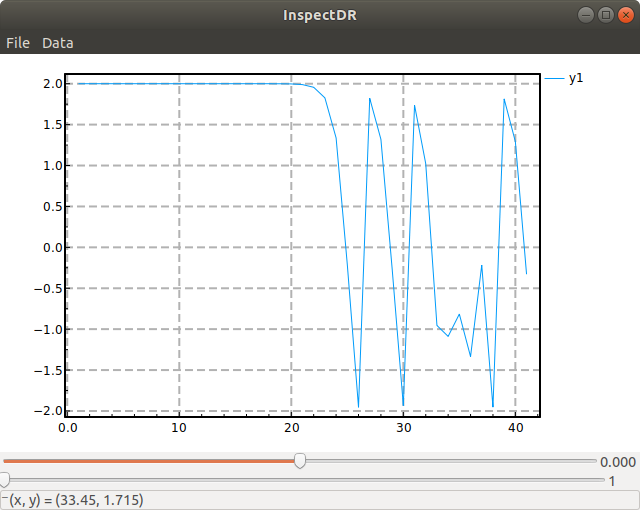
\includegraphics[scale=0.5]{t3.png}
\\
\textit{Wykres ciągu c.}
\\\\
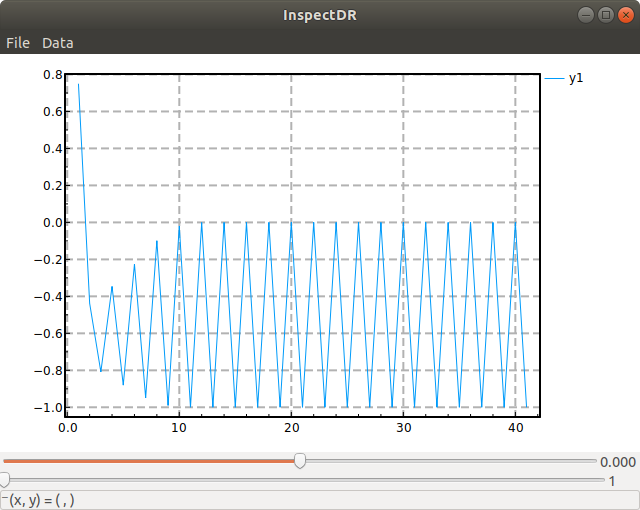
\includegraphics[scale=0.5]{t6.png}
\\
\textit{Wykres ciągu f.}
\\\\
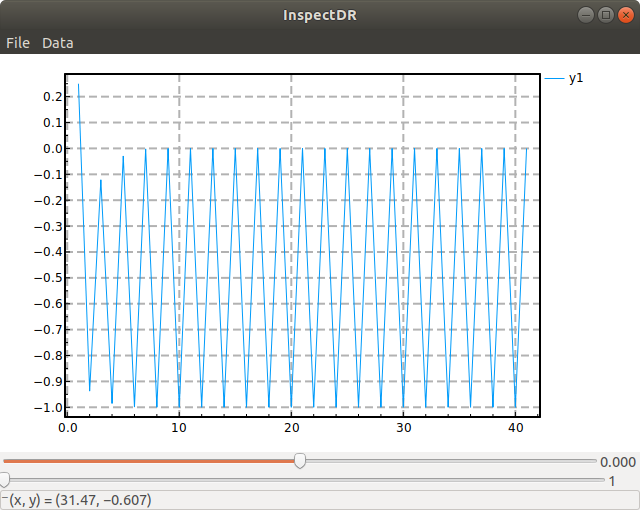
\includegraphics[scale=0.5]{t7.png}
\\
\textit{Wykres ciągu g.}
\\
\subsection{Wnioski}
Dla ciągów \textit{a, b, d, e} iteracje zachowują się stabilnie. Natomiast ciągi \textit{c, f, g} kumulują błedy w kolejnych iteracjach. Przy operacji podnoszenia do kwadratu część cyfr znaczących zostaje utracona. W przypadku ciągu \textit{c} wartości oscylują między -2, a 2, ale nigdy nie występują na tyle blisko tych liczb, żeby zostać do nich zaokrąglone. Ciągi \textit{f, g} są dosyć podobne. Wartości oscylują międy -1, a 0. i w pewnym momencie zostaje popełniony błąd zaokrąglenia $x_n$ do -1. Wtedy ciągi wpadają w pętlę na zmiane zer i minus jedynek.  
\end{document}